\documentclass[letter, 10pt]{article}

%Multicolumna
\usepackage{multirow}

%Pseudo codigo
\usepackage{algpseudocode}

%Cambiado por problemas con tildes
\usepackage[utf8]{inputenc}
\usepackage[spanish]{babel}
\usepackage{amsfonts}
\usepackage{amsmath}

%Cambiado por problemas con tikz
\usepackage{ifpdf}
\ifpdf
    \usepackage{graphicx}  %If run with `pdflatex`
\else
    \usepackage[dvips]{graphicx} %If run with `latex`
\fi


\usepackage{url}
\usepackage[top=3cm,bottom=3cm,left=3.5cm,right=3.5cm,footskip=1.5cm,headheight=1.5cm,headsep=.5cm,textheight=3cm]{geometry}

\usepackage{tikz}
\usetikzlibrary{babel,arrows}

\begin{document}
\title{Inteligencia Artificial \\ \begin{Large}Informe Final: Bus Evacuation Problem\end{Large}}
\author{[Camilo Valenzuela Carrasco]}
\date{\today}
\maketitle


%--------------------No borrar esta secci\'on--------------------------------%
\section*{Evaluaci\'on}

\begin{tabular}{ll}
Mejoras 1ra Entrega (10 \%): &  \underline{\hspace{2cm}}\\
C\'odigo Fuente (10 \%): &  \underline{\hspace{2cm}}\\
Representaci\'on (15 \%):  & \underline{\hspace{2cm}} \\
Descripci\'on del algoritmo (20 \%):  & \underline{\hspace{2cm}} \\
Experimentos (10 \%):  & \underline{\hspace{2cm}} \\
Resultados (10 \%):  & \underline{\hspace{2cm}} \\
Conclusiones (20 \%): &  \underline{\hspace{2cm}}\\
Bibliograf\'ia (5 \%): & \underline{\hspace{2cm}}\\
 &  \\
\textbf{Nota Final (100)}:   & \underline{\hspace{2cm}}
\end{tabular}
%---------------------------------------------------------------------------%

\begin{abstract}
El tema de la evacuación masiva en zonas de riesgo, es un tópico relevante para nuestro país, buscar formas de optimizar dicha evacuación es importantísimo al momento de salvar la mayor cantidad de vidas posible. Una forma de evacuar gente es utilizando los buses del transporte público. En este informe se hablará del Bus Evacuation Problem (BEP), que busca asignar la ruta que debe tomar cada bus con el objetivo de evacuar toda la gente hacia albergues en el menor tiempo posible, teniendo en cuenta la capacidad de los buses y de los albergues. El objetivo de este informe es definir el problema, sus variables y aspectos fundamentales, para luego analizar lo existente en la literatura, definir matemáticamente el problema, y realizar una implementación del problema mediante métodos que no han sido utilizados anteriormente, como son los algoritmos evolutivos.
\end{abstract}

\section{Introducci\'on}
    Luego del huracán Katrina en EE.UU. no se había pensado en la evacuación de personas tránsito-dependientes, que no tienen forma de escapar a los refugios por su cuenta, como por ejemplo las personas de tercera edad y gente con movilidad reducida; ahí es donde surge el Bus Evacuation Problem (BEP) \cite{bish2011planning}. El objetivo es generar rutas que deben tomar los buses, minimizando el tiempo que se demora en evacuar a las últimas personas. Hay que tener en cuenta que los buses disponibles son limitados, y están inicialmente en uno o más terminales de buses, también existen puntos definidos donde los buses tomarán evacuados para luego ser llevados a los distintos refugios que tienen una capacidad limitada.

Poder actuar de manera eficaz y eficiente en situaciones de emergencia es importantísimo para poder salvar vidas, esa es la motivación de estudiar en profundidad el Bus Evacuation Problem. Buscando métodos que nos den respuestas confiables en poco tiempo y estudiar además, distintas variantes del BEP, que tomen en cuenta la incertidumbre que existe en estas situaciones.

El propósito de este documento, es estudiar en detalle el Bus Evacuation Problem, y sentar las bases para proponer una implementación que no ha sido utilizada anteriormente, como es utilizar algoritmos evolutivos para encontrar soluciones al problema.

El presente documento está estructurado en 9 secciones, se comenzará definiendo en profundidad el problema en la sección 2, para luego recopilar los esfuerzos realizados para resolver el problema en la sección 3 mediante un Estado del Arte, en la sección 4 se definirá formalmente el problema utilizando modelos matemáticos, luego en la sección 5 se presentará la representación que se va a utilizará para la propuesta de implementación que se detalla en la sección 6, en la sección 7 se definirán los experimentos utilizados para probar el algoritmo, en la sección 8 se expondrán los resultados de dichos experimentos, para finalizar con las conclusiones en la sección 9.
    
\section{Definici\'on del Problema}
%Explicaci\'on del problema que se va a estudiar, en que consiste, cuales son sus variables, restricciones y objetivos de manera general.
%Variantes m\'as conocidas que existen.

El Bus Evacuation Problem (BEP) definido por \cite{bish2011planning}, se trata de un problema de planificación en estados de emergencia, donde se busca evacuar a una gran cantidad de personas tránsito dependiente -que tienen dificultad para movilizarse por sus propios medios-  de las zonas de riesgo, hacia lugares seguros utilizando buses, con el fin de salvar la mayor cantidad de vidas.

Como se muestra en la Figura \ref{fig:simpleExample} el problema se puede representar como una red, con tres tipos de nodos. Los nodos Y que son los terminales de donde salen los buses; los nodos P son los sectores donde se reúnen las personas que necesitan ser evacuadas; y los nodos S son los refugios donde deberán ser llevados los evacuados.

Existe un conjunto limitado de buses V, que cada uno tiene una capacidad Q de pasajeros; este conjunto se puede dividir en varios subconjuntos $V_i$, $i\in Y$, que contiene los buses que salen del terminal $i$. Cada nodo P tiene una cantidad de personas iniciales $D_i$ , $i \in S$. Cada refugio tiene una capacidad máxima $C_i$ , $i \in S$. Y cada arco entre dos nodos tiene un costo $\tau_{ij}$ , este costo es proporcional al tiempo y la distancia que le toma al bus para llegar desde un nodo $i$ hacia un nodo $j$; además tiene que cumplir ciertas características, como ser no negativo, simétrico ($\tau_{ij} = \tau_{ji}$) y si se pasa por un nodo intermedio tiene que cumplir la desigualdad triangular $\tau_{ij} \leq \tau_{ik} + \tau_{kj}$

Por medidas de seguridad para los choferes, los buses luego de salir de un terminal, no pueden volver a pasar por ningún terminal de buses, y tienen que terminar siempre en un refugio, luego del primer viaje que empieza en un terminal y termina en un refugio, los buses sólo pueden tomar rutas que comienzan en un refugio y terminan en el mismo o en otro refugio. Si un bus llena su capacidad Q y todavía quedan pasajeros en el nodo en que estaba, otro bus puede llegar y tomar a los pasajeros que van quedando hasta que no quede ningúna persona por evacuar.

Lo que se busca es generar las rutas que tiene que tomar cada bus de tal forma de evacuar a toda la gente que está en los distintos sectores de evacuación en el menor tiempo posible; teniendo en cuenta que la evacuación termina cuando las últimas personas en ser evacuadas llegan a algún refugio.

Como resumen tenemos que el BEP tiene como entrada

\begin{itemize}
\item Un conjunto terminales de donde salen los buses Y.
\item Un conjunto de sectores de reunión P.
\item Un conjunto de refugios S.
\item Un vector de buses V, con sus respectivas capacidades.
\item Un vector de demandas en los sectores de reunión D.
\item Un vector de capacidades de refugios C.
\item Una matriz de costos $\tau$.
\end{itemize}

Tenemos las variables de decisión, $x_{ij}^{mt}$ que son variables binarias que toman el valor 1 si en el viaje t el bus m toma atraviesa el camino que va desde i hasta j. Donde i y j pueden ser terminales, sectores de reunión o refugios.

Estas variables están sujetas a las siguientes restricciones:

\begin{itemize}
\item La ruta que toma el bus tiene que respetar el flujo, eso quiere decir que el viaje t+1 tiene que salir del punto final del viaje t.

\item Un bus no puede tomar dos caminos en el mismo viaje.

\item Se tiene que respetar la capacidad máxima de los buses y refugios.

\item Por seguridad de los choferes, luego del primer viaje,  los buses no pueden regresar a los terminales.

\item Se tienen que evacuar a todas las personas de los puntos de encuentro.


\end{itemize}

Y como salida nos debería entregar las rutas que deberían tomar los buses $m \in V$.


Como el BEP es relativamente nuevo, no existen gran cantidad de variantes, algunas buscan además de minimizar el tiempo de evacuación, minimizar el costo total de movilizar los buses \cite{bish2011planning}. Otras variantes tienen que ver con la incertidumbre que existe en la emergencia, uno de ellos toma en cuenta que la cantidad de personas en los distintos puntos no se conoce totalmente, solo se conocen posibles escenarios, y para saber la cantidad de personas que de verdad va a estar en ese punto tiene que pasar un tiempo, y el bus tiene que decidir si esperar para saber en qué escenario está o no esperar y seguir su ruta, este es el Robust Bus Evacuation Problem (RBEP) \cite{goerigk2012robust}, además existen variantes que toman más parámetros como inciertos, como por ejemplo escenarios donde no se sabe la cantidad de personas en los sectores de reunión, los costos van a variar según el tráfico durante la evacuación, la cantidad de buses puede que no sea la inicial, porque algunos van a ser destruidos o no van a estar en funcionamiento en dicho momento y también los refugios pueden haber sido dañados, por lo que sus capacidades han disminuido; teniendo todos esos parámetros inciertos se propuso hacer dos una planificación de dos etapas, una para calcular las rutas y otra para ver que tan vulnerable es la planificación a los problemas relacionados con la emergencia \cite{goerigk2013two}. 


Por otra parte el Bus Evacuation Problem, es un caso especial de otro problema, llamado Vehicle Routing Problem \cite{toth2001vehicle, golden2008vehicle}, este problema no está relacionado con evacuación, sino que está pensado para el sector comercial. Lo que se busca en el Vehicle Routing Problem es satisfacer la demanda por movilización utilizando vehículos, al igual que el BEP, en VRP se busca generar rutas para los vehículos con el objetivo de satisfacer los distintos puntos de demanda, al menor costo (distancia total recorrida) para la empresa. A diferencia del BEP, en el VRP simple, la demanda de un punto tiene que ser servida por sólo un vehículo, no se puede compartir con otros vehiculos, los vehículos solo salen de un punto y llegan al mismo. 

También existen variaciones del VRP \cite{golden2008vehicle , bish2011planning}, donde se agregan puntos intermedios donde pueden descansar los vehículos (que es como tener varios terminales) o demanda compartida. 

\section{Estado del Arte}
%Lo m\'as importante que se ha hecho hasta ahora con relaci\'on al problema. Deber\'ia responder preguntas como las siguientes:
%?`-cuando surge-?, ?`qu\'e m\'etodos se han usado para resolverlo?, ?`cuales son los mejores algoritmos que se han creado hasta
%la fecha?, ?`qu\'e representaciones han tenido los mejores resultados?, ?`cu\'al es la tendencia actual?, tipos de movimientos,
%heur\'isticas, m\'etodos completos, tendencias, etc... Puede incluir gr\'aficos comparativos, o explicativos.\\
%La informaci\'on que describen en este punto se basa en los estudios realizados con antelaci\'on respecto al tema.
%Dichos estudios se citan de manera que quien lea su estudio pueda tambi\'en
% acceder a las referencias que usted revis\'o. Las citas se realizan mediante el comando \verb+\cite{ }+.
%Por ejemplo, para hacer referencia al art\'iculo de algoritmos h\'ibridos para problemas de satisfacci\'on 
% de restricciones \cite{Prosser93Hybrid}.

En esta sección se detalla el inicio del Bus Evacuation Problem (BEP), cual era el contexto en el cual surge este problema. También veremos cómo se relaciona con el Vehicle Routing Problem (VRP), que tiene mayor cantidad de literatura y donde se ha desarrollado más la idea de generar rutas para abastecer cierta demanda. Luego se mostrarán cuales son los métodos que se han utilizado para resolver este problema, y también se verá las propuestas que han realizado otros autores, como variantes del BEP, y cómo abordan soluciones para dichas variantes.

 \subsection{Surgimiento del Bus Evacuation Problem (BEP)}

Luego de la gran destrucción causada por el huracán Katrina el año 2005, se realizaron varios estudios para ver cómo se podrían haber evitado la gran cantidad de muertes luego de dicho evento, uno de ellos \cite{litman2006lessons}, nos habla que gracias a la planificación preventiva, se pudo evacuar gran cantidad de gente, pero este tipo de planificación asociada a emergencias a gran escala a pesar de estar bien documentada e investigada por varios autores \cite{hamacher2001mathematical,cova2003network,chiu2007modeling}, en todos estos modelos no se ha pensado que existe gran cantidad de gente que no tiene las capacidades para evacuar tan fácilmente lugares de riesgo, por ejemplo personas con movilidad limitada y ancianos, a estas personas se les denomina 'tránsito dependientes' ya que necesitan de otra persona para poder evacuar. Según la literatura existen algunos casos donde se aborda la utilización de transporte público  para la evacuación de personas tránsito dependientes \cite{sayyady2010optimizing}, pero no son tan completos como el BEP, ya que por ejemplo no toman en cuenta la capacidad de los refugios donde tienen que evacuar a las personas y no permite que un bus tenga múltiples rutas.  

Es así como el año 2011, surge la idea del Bus Evacuation Problem \cite{bish2011planning}, que busca minimizar el tiempo de evacuación de las personas tránsito dependiente, teniendo en cuenta varias restricciones por ejemplo la cantidad limitada de buses, que todas las personas tienen que ser evacuadas, etc.

\subsection{Bus Evacuation problem (BEP) y el Vehicle Routing Problem (VRP)}

El Vehicle Routing Problem \cite{toth2001vehicle}, trata de un problema donde existen varios puntos de demanda, donde las personas esperan ser transportadas, y se busca generar rutas para satisfacer dicha demanda, minimizando el costo, ya sea de tiempo, distancia o combustible que tienen los distintos vehículos usados para transportar.

Este problema está muy relacionado al BEP, porque los puntos donde se tienen que reunir las personas que necesitan ser evacuadas, tienen cierta demanda, pero el VRP tradicional, no toma en cuenta que los vehículos, en este caso los buses tienen que salir desde una terminal de buses y no pueden volver ninguna terminal, y tampoco toma en cuenta los refugios con capacidad limitada.

Existe una variante del VRP que es la más parecida de BEP llamada 'Split delivery multi-depot vehicle routing problem with inter-depot routes' (SDMDVRPI) que según Bish et al. \cite{bish2011planning} es una mezcla entre varias variantes de VRP.

El SDMDVRPI es una mezcla entre Multi-depot vehicle routing problem with inter-depot routes (MDVRPI) \cite{crevier2007multi}, donde existen varios depósitos donde pueden salir los vehículos a satisfacer demanda, y no necesariamente tienen que volver al mismo depósito  de donde salieron a recargar combustible, sino que pueden llegar a otro para seguir con sus rutas, muy parecido al caso cuando un bus tiene que llegar a un refugio a dejar evacuado y luego puede seguir haciendo rutas, para luego llegar con otros evacuados a otro refugio; con el split delivery vehicle routing problem (SDVRP) \cite{golden2008vehicle}, que cada punto de demanda puede ser visitado más de una vez, por lo que varios buses pueden repartir la demanda de dichos puntos.

\begin{figure}
\centering

\begin{tikzpicture}[->,>=stealth',shorten >=1pt,auto,node distance=3cm,
  thick,yard node/.style={circle,fill=yellow!20,draw,font=\sffamily\Large\bfseries},person node/.style={circle,fill=red!20,draw,font=\sffamily\Large\bfseries}, shelter node/.style={circle,fill=green!20,draw,font=\sffamily\Large\bfseries},
  trans/.style={thick,<->,shorten >=2pt,shorten <=2pt,>=stealth}]

  \node[person node]    (1) {P1};
  \node[person node]    (2) [below of=1] {P2};
  \node[person node]    (3) [below of=2] {P3};
  \node[yard node]      (4) [right of=2] {Y1};
  \node[shelter node]   (5) [left of=1] {S1};
  \node[shelter node]   (6) [left of=3] {S2};
  

  \path[every node/.style={font=\sffamily\small}, trans]
    (1) edge node []    {2} (2)
        edge node []    {5} (5)
        edge node []    {9} (6)
        edge [bend left] node [below left]    {4} (3)
    (2) edge node []    {3} (3)
        edge node []    {6} (5)
        edge node []    {8} (6)
    (3) edge node []    {5} (6)
    (5) edge [bend right] node []    {11} (6);
 \path[every node/.style={font=\sffamily\small},gray!40]
    (4) edge node []    {3} (1)
        edge node []    {4} (2)
        edge node []    {6} (3);
\end{tikzpicture}


\caption{Ejemplo Simple de Bus Evacuation Problem (BEP) como una red. Fuente: \cite{bish2011planning}}
\label{fig:simpleExample}
\end{figure}

\begin{figure}
\centering
\begin{tikzpicture}[->,>=stealth',shorten >=1pt,auto,node distance=3cm,
  thick,yard node/.style={circle,fill=yellow!20,draw,font=\sffamily\Large\bfseries},person node/.style={circle,fill=orange!20,draw,font=\sffamily\Large\bfseries}, shelter node/.style={circle,fill=blue!20,draw,font=\sffamily\Large\bfseries},
  trans/.style={thick,<->,shorten >=2pt,shorten <=2pt,>=stealth}]

  \node[person node]    (1) {P1};
  \node[person node]    (2) [below of=1] {P2};
  \node[person node]    (3) [below of=2] {P3};
  \node[shelter node]   (5) [left of=1] {Y/S};
  \node[shelter node]   (6) [left of=3] {Y/S};
  

  \path[every node/.style={font=\sffamily\small}, trans]
    (1) edge node []    {2} (2)
        edge node []    {5} (5)
        edge node []    {9} (6)
        edge [bend left] node [below left]    {4} (3)
    (2) edge node []    {3} (3)
        edge node []    {6} (5)
        edge node []    {8} (6)
    (3) edge node []    {5} (6)
    (5) edge [bend right] node []    {11} (6);
\end{tikzpicture}


\caption{Ejemplo de SDMDVRPI como una red (Y/S se refiere a un depósito de vehículos y los nodos P son puntos de demanda). Fuente: \cite{bish2011planning}}
\label{fig:SDMDVRP}
\end{figure}

A diferencia del BEP (Figura \ref{fig:simpleExample}) en el SDMDVRP sólo existen dos tipos de nodos, los depósitos de vehículos y los puntos de demanda (Figura \ref{fig:SDMDVRP}), además el objetivo de SDMDVRP es obtener el menor costo, en contraste del BEP que tiene un objetivo min-max, que busca minimizar el máximo tiempo que se demora un bus en evacuar, esto quiere decir que el óptimo es cuando el tiempo que se evacua a las últimas personas es el mínimo.

\newpage
\subsection{Encontrando una solución al BEP}

El Bus Evacuation Problem ha tenido dos acercamientos para obtener soluciones, el primero es inherente al tipo de modelo matemático utilizado para representar el problema, que se trata de un modelo MIP (Mixed Iteger programming) \cite{bish2011planning,goerigk2012robust,goerigk2013two}, donde se utiliza programación lineal para obtener una solución óptima. El otro acercamiento es mediante algoritmos heurísticos, que no necesariamente encuentran el óptimo, pero son más veloces y pueden encontrar soluciones a instancias del problema mucho más grandes que en el caso de programación lineal.

\subsubsection{Programación lineal}

Definiendo el BEP como un modelo MIP, se pueden encontrar soluciones óptimas que minimizan el tiempo de evacuación para escenarios pequeños utilizando métodos de programación lineal, como simplex; pero cuando dichos escenarios comienzan a crecer (por ejemplo una gran cantidad de nodos en la red), encontrar la solución óptima cada vez es más costoso. Por lo que algunos autores, además del tiempo de evacuación, buscan minimizar el costo o distancia que recorren los buses \cite{bish2011planning}, para esto cambian la función objetivo del modelo, agregando una constante de lexicográfica, para dar mayor prioridad al tiempo de evacuación o al costo de los buses, pero tratando de minimizar ambas. Un ejemplo de función objetivo sería.
\begin{equation*}
  \text {Minimize }T_{evac} + \frac{1}{L} \left( \sum_{(i,j) \in A} \sum_{m \in V} \sum_{t = 1}^T \tau_{ij} x_{ij}^{mt} \right)
\end{equation*}

Donde $T_{evac}$ es el tiempo de evacuación total, L es la constante lexicográfica, A son los arcos entre los nodos de la red, V es el vector de buses, T es la cantidad máxima de viajes, $\tau$ es la matriz de costos asociada a los arcos y  $x_{ij}^{mt}$ es una variable binaria que dice si el bus m tomó el arco (i,j) en el viaje t.

Al agregar el costo de los viajes, se busca hacer que los buses realicen la menor cantidad de recorridos, con el fin de evacuar a las personas, el tiempo de evacuación puede aumentar un poco encontrando una solución cercana al óptimo, pero las rutas que eran demasiado caras ya no son tomadas, y la optimización se realiza más rápido.

Otra forma de agilizar el proceso de buscar soluciones, utilizar una heurística, que divide el problema en dos subproblemas \cite{bish2011planning}. El primero es encontrar las distintas rutas posibles en la red, ya sea desde un terminal de buses, pasando por puntos de reunión de evacuados, y luego terminar en un refugio, o las rutas que comienzan en un refugio, toman evacuados de los puntos de reunión y vuelven a otro o el mismo refugio. Luego de tener todas las rutas tenemos que decidir que decir que bus va a tomar qué rutas, pensando que pueden tomar más de una. Por lo que se puede generar un nuevo modelo, que no construye las rutas, sino que sólo decide que bus va a tomar qué ruta. Este segundo modelo también puede ser utilizado con programación lineal, pero se necesita tener un vector de rutas R y puede ser que el resultado sólo es cercano al óptimo, pero se puede arreglar este resultado utilizando algoritmos heurísticos. No se han realizado análisis de este modelo utilizando programación lineal, pero al reducir el espacio de búsqueda, al elegir que ruta toma cada bus en cada recorrido, en vez de decidir arco por arco cúal es el mejor, la optimización tenderá a ser mucho más rápida.

\subsubsection{Algoritmos Heurísticos}
Existen varios algoritmos heurísticos para este problema, que buscan encontrar soluciones cercanas al óptimo, algunos buscan construír soluciones y otros buscan arreglar soluciones ya construídas.

\paragraph{Heurística 1}

El primer algoritmo heurístico propuesto \cite{bish2011planning} se divide en dos fases, la primera fase busca generar una solución factible del problema, y se divide en tres pasos.
\begin{itemize}
\item \textbf{Paso 1:} Se produce una lista de buses ordenada en un orden no-decreciente de la cantidad de movimientos que tiene que hacer el bus desde un terminal de buses $Y_j$ o un refugio $S_j$ a un lugar de reunión de evacuados $P_j$ más la cantidad de movimientos que tiene que hacer desde un punto de reunión $P_j$ hacia un refugio $S_j$. Esta lista, en segundo lugar tiene que estar ordenada por el costo total asignado al bus para cuando existen buses con la misma cantidad de movimientos. (Inicialmente el número de movimientos y el costo de cada bus es cero).  
\item \textbf{Paso 2:} Se toma el primer bus de la lista. Si ese bus está en un sector de reunión $P_j$ se tiene que generar una ruta hacia el refugio con capacidad suficiente para dejar a todos los pasajeros, si el bus está en un terminal $Y_j$ o en un refugio $S_j$ se debe generar una ruta hacia el punto de reunión de evacuados $P_j$ más cercano con personas esperando a ser rescatadas, cuando llega a ese punto tiene que ver si le queda capacidad para llevar más personas, si es así tiene que seguir a otro punto de reunión para recoger personas hasta que se llene la capacidad del bus. Luego de realizar la ruta del bus, hay que actualizar la lista de buses, agregando los cambios realizados al bus que se tomó de la lista; esto quiere decir cambiar la cantidad de movimientos necesarios para llegar a un refugio o a un punto de reunión, y el costo acumulado que lleva ese bus.

\item \textbf{Paso 3:} Se tiene que volver al Punto 1, hasta que todas las personas sean evacuadas.
\end{itemize}

La idea de tomar el primer bus de la lista ordenada por mayor cantidad de movimientos, es que en cada iteración se buscan las rutas con menor costo y se asignan a los buses que llevan el mayor costo acumulado, dejando los costos de los buses equilibrados.

Luego de obtener una solución factible en la primera fase, la segunda fase busca tratar de mejorar esta solución, para llegar a algún resultado cercano al óptimo. Esta segunda fase se divide en 6 pasos.

\begin{itemize}
\item \textbf{Paso 1:} Seleccionar el bus con mayor costo acumulado, ya que este es el que hay que cambiar para optimizar el $T_{evac}$. Lo que se tiene que realizar es intercambiar la primera ruta asignada al bus seleccionado, por la primera ruta asignada al bus con menor costo.

\item \textbf{Paso 2:}  Verificar que el cambio de rutas entre el bus con mayor costo y el con menor costo, genera una reducción del $T_{evac}$ y mantiene la factibilidad de la solución. Si es así, actualizar la lista de costo de los buses y volver a realizar el paso 1, para seguir intercambiando rutas de los buses más costosos. Si el $T_{evac}$ es mayor o la solución luego del intercambio no es factible, seguir al paso 3.

\item \textbf{Paso 3:} Como no se puede utilizar la primera ruta del bus con menor costo, vemos si ese bus tiene otra ruta para ser intercambiada, si es así volvemos al paso 2, si no vamos al paso 4.

\item \textbf{Paso 4:} Ver si la primera ruta del bus con mayor costo puede ser asignada como la última ruta del bus del menor costo, reduciendo el $T_{evac}$. Si es así se reasigna la ruta al otro bus, y se actualiza la lista de buses con sus costos, y se vuelve al paso 1, si no se puede reasignar la ruta al bus con menor costo, seguimos con el paso 5.

\item \textbf{Paso 5:} Tomamos el bus con el segundo menor costo y tratamos de intercambiar su primera ruta con el bus de mayor costo, volviendo al paso 2. Si no hay más buses se tiene que ir al paso 6.

\item \textbf{Paso 6:} Como no se encontró ningún intercambio para la primera ruta del bus con mayor costo, ahora la ruta a intercambiar de ese bus es la segunda de mayor costo, si es que existe dicha ruta se vuelve al paso 2, intentando intercambiar esta ruta, si no existe dicha ruta, se termina el algoritmo.
\end{itemize}

\paragraph{Heurística 2}

Otro algoritmo heurístico, utiliza el segundo modelo presentado por Bish et al. \cite{bish2011planning} donde se necesita precalcular las distintas rutas posibles de la red. Este segundo algoritmo tiene 3 pasos.

\begin{itemize}
\item \textbf{Paso 1:} Utilizar el primer algoritmo heurístico o cualquier heurística que nos entregue una solución factible del BEP, y determinar las rutas utilizadas por los distintos buses.

\item \textbf{Paso 2:} Resolver mediante programación lineal una versión relajada del problema, quitando la restricción de que las variables de decisión sean enteras. Así encontraremos otro conjunto de rutas que pueden tomar los buses.

\item \textbf{Paso 3:} Como ahora se tiene un gran conjunto de rutas para ser asignadas a buses, primero se eliminan las rutas duplicadas, y ahora se pueden utilizar estas rutas para el segundo modelo, inicializando las variables de decisión en una solución en una solución generada en el paso 1.
\end{itemize}

Estos dos primeros algoritmos fueron pensados para trabajar en conjunto, el primero no siempre llega a una solución óptima, pero luego es arreglado mediante el segundo algoritmo heurístico, llegando a una solución mucho más cercana al óptimo, que en el caso de la literatura era un óptimo conocido. También se puede observar que el primer algoritmo busca construir una solución, y el segundo comienza de una solución factible, y busca optimizarla.

%\textbf{Branch and Bound}

%Otro acercamiento heurístico es utilizando el framework Branch and Bound para encontrar una solción óptima \cite{goerigk2013branch} 


\subsection{Robust Bus Evacuation Problem}

Una de las variantes del BEP, es el Robust Bus Evacuaton Problem (RBEP), donde se agrega incertidumbre a algunas variables del problema, por ejemplo la cantidad de gente que está esperando en cada punto de reunión. No son modelos estocásticos, donde se toma en cuenta probabilidades sobre los datos que se le entregan al modelo, sino que el modelo robusto, toma en cuenta varios escenarios posibles.


\subsubsection{Robust Bus Evacuation with delayed scenario information.}
En este problema, la cantidad de personas que se encuentra en cada punto de reunión no se sabe al comenzar la evacuación, solo se conoce una lista de posibles escenarios, que nos dicen la cantidad esperada de personas en cada punto \cite{goerigk2012robust}. Luego de un tiempo $p_{wait}$, se sabe en qué escenario uno se encuentra, si no espera dicho tiempo, no puede volver hasta terminar su ruta. 

En este tipo de problema además de generar la ruta que tienen que tomar los buses, hay que decidir si el bus va a esperar $p_{wait}$ a que llegue toda la gente que se espera, o si no espera y parte, teniendo que volver si es que hay más gente esperando.

Para este tipo de problema se generó un modelo mixto, con variables continuas y enteras, y se utilizaron dos métodos para resolverlos.

\paragraph{Búsqueda Lineal}
El primer método es realizar una búsqueda lineal, para ver cual es la mejor combinación de buses que esperan y que no esperan, que optimiza el tiempo. Para esto se resuelve un modelo mixto reducido del problema y se resuelven $|B| + 1$, de estos modelos utilizando programación lineal, con $|B|$ la cantidad de buses.

Este método recorre todas las posibilidades y encuentra soluciones factibles, para luego entregar la mejor de ellas.

\paragraph{Búsqueda Tabú}

La idea de la búsqueda tabú, es tomar en cuenta las soluciones ya visitadas cuando se realiza una búsqueda local que mejore la solución en la que se está actualmente.

\subparagraph{Representación de la solución}

Para representar la solución de nuestro problema se generará una tabla con los distintos tours que toma cada bus. Cada tour se representa como un par ordenado, entre un punto de reunión y un refugio, por ejemplo el par (1,3) representa un tour completo donde tomamos evacuados en el punto de reunión 1 y los dejamos en el refugio 3.

\subparagraph{Movimientos Locales}

Para realizar la búsqueda se necesita definir los movimientos que se pueden realizar a una solución para poder realizar una búsqueda local. 


\begin{itemize}
\item \textbf{Movimiento 1:} Modificar un tour: Se toma un tour de la solución actual (p,s) y se cambia por algún otro (p',s'). $p\in P$ , $s \in S$.

\item \textbf{Movimiento 2:} Agregar un tour: Se agrega un tour a un bus.

\item \textbf{Movimiento 3:} Borrar un tour: Se quita un tour de algún bus, algún bus puede quedar sin tours.

\item \textbf{Movimiento 4:} Agregar un bus: Ya sea agregar un bus que no espera, con solo un tour, o agregar un bus que espera que llegue la gente y agregar un tour por cada escenario posible.

\item \textbf{Movimiento 5:} Quitar un bus: Eliminar el bus y todos los tours asociados.

\item \textbf{Movimiento 6:} Mover tour: Quitar el último tour de algun bus, y asignarlo a otro. 

\item \textbf{Movimiento 7:} Cambiar el tipo de bus: Cambiar de un bus que no espera, a un bus que espera la llegada de gente.

\item \textbf{Movimiento 8:} Intercambiar tours: tomar un tour de algún bus y cambiarlo por algún otro tour de otro bus.
\end{itemize}

Al aplicar alguno de estos movimientos a nuestra solución, realizamos una búsqueda local en el vecindario de la solución actual y cada vez que se realiza un movimiento se agrega a una lista tabú para no volver a la solución anterior. Si al realizar un movimiento, todas las soluciones vecinas son infactibles o los tiempos de evacuación son mayores a la solución inicial, estamos en un óptimo, pero podría ser un óptimo local, por lo que dejamos a la solución que tome un valor infactible o un valor mayor, para poder salir de ese óptimo local, para esto se define una nueva función objetivo de la búsqueda.

$$ obj_{tabu} = T_{evac} +  p_{sat} inf^{sat} + p_{cap} inf^{cap} + p_{bus} inf^{bus}$$

Los valores de $ inf^{sat}$,$ inf^{cap}$,$ inf^{bus}$, son la cantidad de personas que no pueden ser evacuadas, violaciones a la capacidad de los refugios, y el número de buses de más que se utilizaron, respectivamente en todos los escenarios posibles.

Por otra parte  $p_{sat}$, $ p_{cap}$,$ p_{bus}$, son parámetros de castigo, por haber violado alguna de las restricciones, estos parámetros van aumentando a medida que se encuentran más soluciones infactibles y disminuye si se encuentran soluciones factibles.

Luego de una cantidad de iteraciones que no se encuentren soluciones factibles del problema, la búsqueda se reinicia, limpiando la lista tabú y volviendo los parámetros de castigo a su valor inicial.

Para iniciar la búsqueda se necesita generar una solución factible, para esto se utiliza un método greedy, donde se usan dos buses, el primer bus no espera pasajeros, realiza tours tomando la mínima cantidad de personas en cada punto de reunión. Luego se realiza un plan de viaje del segundo bus para cada escenario, evacuando la gente que no evacuó el primer bus. Esto nos entrega una solución factible, en tiempo polinomial, que luego se entrega a la búsqueda tabú para ser mejorada, agregando más buses y cambiando los planes de viaje para mejorar el tiempo de evacuación.

Luego de realizar la búsqueda tabú obtendremos la mejor solución factible encontrada, que no necesariamente es el óptimo, pero se realiza en un tiempo menor que resolver utilizando programación lineal o la búsqueda lineal propuesta anteriormente.

\subsubsection{Two-stage Robustness Approach.}

En esta propuesta \cite{goerigk2013two}, toman en cuenta que todos los parámetros en el momento de la emergencia pueden ser inciertos. En este caso existe una gran cantidad de escenarios posibles que llamaremos $U$, este conjunto tiene todos los escenarios posibles, que son finitos, pero son una gran cantidad. En este tipo de situaciones tenemos dos opciones simples para encontrar una solución, encontrar una que sea factible en todos los escenarios, o que sea la mejor solución para el peor escenario. Puede ser que ninguno de estos tipos de solución sea la mejor, pero como no sabemos en qué escenario estamos, no podemos encontrar un óptimo al primer intento. 

Este acercamiento de dos etapas nos dice que cuando no estamos en emergencia podemos generar una solución, de tal forma que en el momento de la emergencia, cuando ya se sepa en qué escenario se encuentra, realizar la menor cantidad de cambios a nuestra solución que en ese momento puede ser infactible y convertirla en una buena solución factible. Para esto se tiene que realizar un modelo robusto del problema, que tome en cuenta los distintos escenarios posibles $RP(U)$, con $U$ el conjunto de escenarios posibles.

Por la gran cantidad de escenarios que existen para cada instancia del problema, resolverlo mediante un software de Programación Lineal, no es muy conveniente, por lo que se realizó un algoritmo iterativo.

\paragraph{Oracle-Base Algorithm}
Se busca generar dos soluciones, la primera corresponde a la primera etapa , la de planificación ($x$), y la segunda dependerá de cada escenario $(x^\xi)_{\xi \in U}$, para esto se utiliza una funcion Oráculo, que dada un conjunto de soluciones $(x,x^\xi)_{\xi \in U'}$ de un subconjunto de los escenarios posibles $U' \subseteq U$, busca el peor escenario donde se necesite modificar mucho la solución, para llegar a una solución factible en dicho escenario.

Se comienza el algoritmo resolviendo el modelo robusto del BEP (RP), con $RP(\emptyset)$, obtenemos el resultado de un BEP normal con solución $(x^{(0)},x^{(0),\xi}) $,, en cada iteración pedimos el peor escenario para nuestra solución $\xi = \omega((x^k , x^{k,\xi}))_{\xi \in U'}$, con $\xi \in U$ y $U' \subseteq U$. Luego resolvemos el modelo $RP(U'^{k+1})$ robusto con $U'^{k+1} = U'^{k} \cup \xi$, y así obtenemos la solución $(x^k, x^{k,\xi})$. Se itera hasta incluir los escenarios que uno necesite.


\section{Modelo Matem\'atico}
%Uno o m\'as modelos matem\'aticos para el problema.
Existe un modelo de este problema utilizado ampliamente en la literatura, de éste modelo base surgen otros modelos, utilizando algunos métodos como por ejemplo entregarle al problema todas las rutas posibles, y encontrar sólamente que bus toma que ruta, todo esto, para reducir el espacio de búsqueda, o se le agregan cambios a la función objetivo, también los modelos del Robust Bus Evacuation Problem toman como base este modelo.

Tomando en cuenta lo dicho en la sección Definición del Problema y utilizando el modelo propuesto por \cite{bish2011planning}, se necesitan como parámetros, un conjunto terminales de donde salen los buses Y; un conjunto de sectores de reunión P; un conjunto de refugios S; un vector de buses V, con sus respectivas capacidades Q; un vector de demandas en los sectores de reunión D; un vector de capacidades de refugios C; una matriz de costos $\tau$ y los arcos que conectan los nodos A.

También se definen las siguientes variables de decisión del problema .

\begin{itemize}
\item $x_{ij}^{mt}$: Variable binaria, que toma el valor de 1 si en el viaje t el bus m atraviesa el arco (i,j). Si no es así esta variable toma el valor cero. $\forall (i,j) \in A$, $m \in V$, $t = 1,\dots,T$.
\item $b_j^{mt}$: Número de personas evacuadas desde el punto de reunión j (o dejadas en el refugio j) asignadas al bus m luego del viaje t. $\forall j \in (P \cup S)$, $m \in V$, $t = 1,\dots,T$.
\item $T_{evac}$: Tiempo de evacuación.
\end{itemize}

Utilizando estas variables de decisión se puede modelar el problema.

\begin{align}
\text{Minimize }& T_{evac}\\
\text{sujeto a: }& T_{evac} \geq  \sum_{(i,j) \in A}  \sum_{t=1}^T \tau_{ij} x_{ij}^{mt}, \forall m \in V\\
&  \sum_{i:(i,j) \in A} x_{ij}^{mt} =  \sum_{k:(j,k)\in A} x_{jk}^{m(t+1)}, \forall j \in P, m \in V, t = 1,\dots,T-1\\
&  \sum_{i:(i,j) \in A} x_{ij}^{mt} \geq  \sum_{k:(j,k)\in A} x_{jk}^{m(t+1)}, \forall j \in S, m \in V, t = 1,\dots,T-1\\
&  \sum_{(i,j) \in A} x_{ij}^{mt} \leq 1, \forall m \in V, t = 1, \dots, T\\
& x_{ij}^{m1} = 1, \forall i \in Y, j:(i,j)\in A, m \in V_i\\
& x_{ij}^{mt} = 0, \forall i \in Y, j:(i,j) \in A, m \in V, t = 2,\dots,T\\
& x_{ij}^{mT} = 0, \forall j \in P, i:(i,j)\in A,m\in V\\
&b_j^mt \leq  \sum_{(i,j)\in A} Q x_{ij}^{mt}, \forall j \in (P \cup S), m \in V , t = 1,\dots,T\\
&0 \leq  \sum_{j \in P}  \sum_{\text{l=1}}^t b_j^{ml} -  \sum_{k \in S}  \sum_{l=1}^t b_k^{ml} \leq Q, \forall m \in V, t = 1, \dots , T\\
&\sum_{m\in V}  \sum_{t = 1}^T b_j^{mt} \leq C_j, \forall j \in S\\
& \sum_{m \in V}  \sum_{t=1}^T b_k^{mt} = D_j, \forall j \in P\\
& \sum_{j\in P}  \sum_{t = 1}^T b_j^{mt} =  \sum_{k\in S}  \sum_{t = 1}^T b_k^{mt}, \forall m \in V\\
&x_{ij}^{mt} \in {0,1}, \forall (i,j) \in A, m\in V, t = 1,\dots,T\\
& b_k^{mt} \geq 0, \forall (i,j) \in A, m \in V, t = 1,\dots,T
\end{align}


El objetivo es minimizar el tiempo de evacuación (1), y ese tiempo del bus que se demora más (o con mayor costo) en evacuar (2). La restricción (3) tiene que ver con el flujo de la red, para mantenerlo el viaje en el tiempo t+1 tiene que empezar del nodo donde estaba en el tiempo t, en el caso de estar en un refugio puede ser que un bus no vuelva a salir del refugio por lo que se utiliza otra restricción (4). La restricción (5) nos asegura que un bus puede realizar sólo un viaje a la vez. Las restricciones (6) y (7) son para que sólo en el primer tiempo los buses puedan salir desde un terminal de buses, luego de ese tiempo no pueden volver a ningún terminal. La restricción (8) es para la seguridad de los choferes de los buses, ya que limita a que en el último tiempo, el bus tiene que llegar a un refugio. La restricción (9) nos dice que un bus sólo puede tomar pasajeros en un nodo j, si el bus está en ese nodo. La restricción (10) limita la capacidad del bus. La restricción (11) limita la cantidad de personas que pueden ser dejadas en los refugios, y la (12) nos dice que todas las personas que están esperando en los puntos de reunión tienen que ser evacuados. La restricción (13) es para que todos los evacuados lleguen a un refugio. Para finalizar las restricciones (14) y (15) tienen que ver con la naturaleza de las variables de decisión, binaria para x y no negativa para b. 

Un ejemplo de alguna variante de este modelo es el utilizado en los algoritmos heurísticos de \cite{bish2011planning}. En este modelo se divide el problema de generar las rutas y asignar dichas rutas a los distintos buses, pre calculando las rutas posibles y entregando esas rutas al modelo para que las asigne a los distintos buses.

En este modelo necesitamos un conjunto de rutas R, y se agregan tres indicadores binarios como parámetros, $s_{rj}$, $\forall r \in R$, $j \in Y \cup S$, que vale 1 si la ruta r comienza en el terminal o refugio j, 0 si no es así; $v_{rj}$ , $\forall r \in R$, $j \in P$, es 1 si la ruta r visita el nodo j y $e_{rj}$ , $\forall r \in R$, $j \in Y\cup S$, que vale 1 si la ruta r termina en el terminal o refugio j. Con estos nuevos parámetros tenemos que definir unas nuevas variables de decisión.

\begin{itemize}
\item $\hat{x}_r^{mt}$: Variable binaria que vale 1 si el bus m es asignado a la ruta r en el tiempo t, sino vale 0. $\forall r \in R$, $m\in V$, $t = 1, \dots,T$.
\item $\hat{b}_j^{mt}$: Número de evacuados del nodo j por el bus m en el tiempo t, $\forall j \in P \cup S$, $m \in V$, $t = 1,\dots,T$
\end{itemize}

Además en vez del costo entre nodos se utilizará el costo total de la ruta que lo denotaremos como $\hat{\tau}$. Utilizando lo definido anteriormente y agregando el orden lexicográfico de la sección 3.3.1, se obtiene el siguiente modelo .

\begin{align}
\text{Minimize }& T_{evac} + \frac{1}{L}\sum_{r\in R} \sum_{m\in V} \sum_{t=1}^T t \hat{x}_r^{mt}\\
\text{sujeto a: }& T_{evac} \geq  \sum_{r \in R}  \sum_{t=1}^T \hat{\tau}_{r} \hat{x}_{r}^{mt}, \forall m \in V\\
& \sum_{r\in R} s_{ri} \hat{x}_r^{m1} = 1, \forall i \in Y, m \in V_i\\
& \sum_{r \in R} s_{ri} \hat{x}_r^{mt} = 0, \forall i \in Y, m \in V, t = 2,\dots,T\\
& \sum_{r \in R} \hat{x}_r^{mt} \leq 1, \forall m \in V, t = 1,\dots, T\\
& \sum_{r \in R} s_{rs} \hat{x}_r^{m(t+1)} \leq \sum_{r \in R} e_{rs} \hat{x}_r^{mt}, \forall s \in S, m \in V, t = 1, \dots, T-1
\end{align}
\begin{align}
&\hat{b}_j^{mt} \leq Q \sum_{r\in R} v_{rj} \hat{x}_r^{mt}, \forall j \in P , m \in V, t = 1,\dots,T\\
&\hat{b}_j^{mt} \leq Q \sum_{r\in R} e_{rj} \hat{x}_r^{mt}, \forall j \in S , m \in V, t = 1,\dots,T\\
&\sum_{j \in P} \hat{b}_j^{mt} \leq Q, \forall m \in V, t = 1,\dots,T\\
&\sum_{j \in S} \hat{b}_j^{mt} \leq Q, \forall m \in V, t = 1,\dots,T\\
&\sum_{m \in V} \sum_{t = 1}^T \hat{b}_j^{mt} \leq C_j, \forall j \in S\\
&\sum_{m \in V} \sum_{t = 1}^T \hat{b}_j^{mt} = D_j, \forall j \in P\\
&\sum_{s \in S} \hat{b}_s^{mt} = \sum_{j \in P} \hat{b}_j^{mt}, \forall m \in V, t = 1,\dots,T\\
& \hat{x}_r^{mt} \in {0,1}, \forall r \in R, m \in V, t = 1,\dots,T\\
&\hat{b}_j^{mt} \geq 0, \forall j \in P \cup S, m \in V, t = 1,\dots,T
\end{align}

En este caso se busca casi lo mismo que en el modelo anterior, pero al agregar el segundo término a la función objetivo ahora no se toman en cuenta rutas innecesarias o demasiado caras. La restricción (18) nos dice que la primera ruta tiene que comenzar en un terminal de buses, y la restricción (19) nos limita a que después de la primera ruta no se puede volver a utilizar una ruta que comience de un terminal. La restricción (20) es para que un bus solo pueda hacer una ruta a la vez. La restricción (21) tiene que ver con el flujo de las rutas, uno tiene que haber llegado un refugio, para luego comenzar una ruta desde el mismo refugio. Las restricciones (22) y (23) nos dicen que el bus tiene que visitar un punto de reunión para tomar pasajeros y debe llegar a un refugio para dejarlos. Las restricciones (24) y (25) tienen que ver con la capacidad máxima del bus. La restricción (26) limita la capacidad de los refugios. La restricción (27) nos dice que se tiene que evacuar a todas las personas y la restricción (28) nos dice que todos los evacuados luego de ser tomados en un punto de reunión tienen que ser dejados en un refugio. Las restricciones (29) y (30) tienen que ver con la naturaleza de las variables de decisión.

Estos dos modelos son los más utilizados como base para los distintos algoritmos y variantes que se encuentran en la literatura del BEP.

\section{Representaci\'on}
Al momento de implementar un algoritmo para encontrar soluciones del Bus Evacuation Problem (BEP), hay que tener en cuenta cómo se representa matemáticamente la solución, para luego llevar esa representación a algo más útil para ser manipulado por el algoritmo sin perder información, pensando que utilizaremos un algoritmo evolutivo, tenemos una mayor flexibilidad al momento de elegir las estructuras de datos que se utilizarán para representar la solución. 

La representación matemática del Bus Evacuation Problem (BEP) son variables binarias de la forma $x_{ij}^{mt}$, que toman el valor 1 cuando el bus m toma el camino que va desde i a j en el tour t. Al ser variables binarias con 4 índices, el espacio de búsqueda aumenta exponencialmente al agregar buses, tours o caminos, por lo que utilizar esta representación no se vuelve conveniente al momento de implementar el algoritmo.

Al momento de pensar en las estructuras de datos que fueron utilizadas para el algoritmo, se tomaron en cuenta varios puntos importantes. Primero se pensó en tener toda la información que ofrece la representación matemática, por lo que se utilizó una lista de buses y cada elemento de la lista contenia una lista de los caminos utilizados por el bus. También se pensó en las restricciones del problema, por lo que la lista de caminos está dividida en dos.

\begin{enumerate}
    \item Un tour inicial, que comienza en un terminal, pasa por un punto de reunión y termina en un refugio. Utilizando esta estructura podemos controlar que sólo el primer camino tomado por el bus comienza en un terminal y luego no se puede volver a un terminal.

    \item Una lista de Rutas, donde en cada Ruta se visita un punto de encuentro y se evacuan personas hacia un refugio. De esta forma se puede controlar el flujo de los buses. El bus siempre sale del refugio de la Ruta anterior, pasa por el punto de la ruta actual y deja los evacuados en el refugio de la ruta actual. 
    
\end{enumerate}

Para el desarrollo del algoritmo se utilizó el lenguaje de programación C y se utilizaron estructuras anidadas para representar la solución de la forma expuesta anteriormente, como se muestra en la Figura \ref{fig:representacion}.

Los valores utilizados para Terminal de Salida, Punto Visitado y Refugio, son los valores pertenecientes a los conjuntos Y (Terminales), P (Puntos de reunión), S (Refugio) respectivamente, y están relacionados con los índices i,j de la representación matemática. A su vez el índice utilizado para acceder a algún bus de la lista de buses, está relacionado al indice m de la representación matemática. También se puede relacionar el Tour inicial y El indice de la Ruta en la Lista de rutas con el índice t de la representación matemática. En resumen podemos decir que los valores que tenemos en la estructura de datos serían las variables de la representación matemática que tienen valor 1.

\begin{figure}
\centering
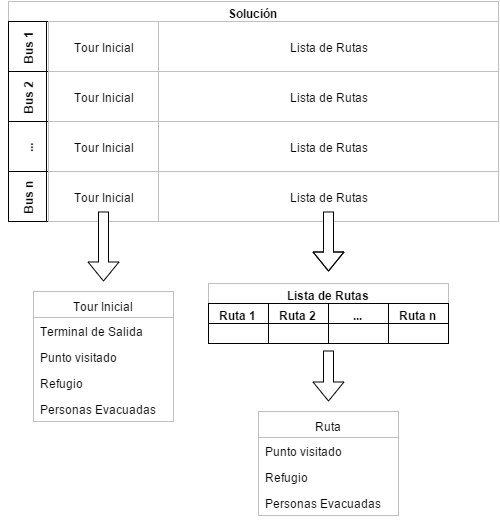
\includegraphics[scale=0.5]{Representacion.png}
\caption{Estructuras de Datos Utilizadas por el algoritmo. Fuente: Elaboración Propia}
\label{fig:representacion}
\end{figure}

\section{Descripci\'on del algoritmo}
%C\'omo fue implementando, interesa la implementaci\'on m\'as que el algoritmo gen\'erico, es decir,
%si se tiene que implementar SA, lo que se espera es que se explique en pseudo c\'odigo la estructura
%general y en p\'arrafo explicativo cada parte como fue implementada para su caso particular, si
%se utilizan operadores se debe explicar por que se utiliz\'o ese operador, si fuera el caso de una
%t\'ecnica completa, si se utiliza recursi\'on o no, etc. En este punto no se espera que se incluya
%c\'odigo, eso va aparte.


Luego de tener pensadas las estructuras de datos a utilizar, se comenzó con la implementación del algoritmo evolutivo, esta implementación estuvo dividida en diversas etapas donde se generaban pequeños modulos, con funcionalidades específicas, y luego se agregaban al algoritmo principal.

\subsection{Inicializando Población}
    Como todo algoritmo evolutivo, contamos de una población de soluciones o individuos. En la implementación del algoritmo se pensó en 2 formas de inicializar la población. En ambas se tiene en cuenta la restricción de buses por terminal, por lo que al comienzo se van fijando los terminales de donde salen los buses en la estructura del Tour Inicial, luego sólo nos preocupamos de asignar el punto donde va a pasar el bus y el refugio donde dejará los evacuados.
    
    La primera forma de inicializar la población, solo tomabamos en cuenta el Tour Inicial de cada bus, luego de fijar los terminales, se toma un punto aleatorio para el Tour Inicial de cada bus y se deja los evacuados en Refugios aleatorios, luego se repite esta operación para cada solución de nuestra población, creando soluciones infactibles del problema. La idea era que los operadores evolutivos se encargaran de asignar aleatoriamente más rutas a los buses, pero al ser todo tan aleatorio, puede ser que pasara por puntos que ya no tuviesen gente por evacuar o deje personas sin evacuar en algunos puntos , por lo que no se utilizó esta forma de inicializar en el algoritmo final.
    
    La segunda forma que se pensó fue ir punto por punto evacuando personas a refugios que tuviesen capacidad, tomando el primer punto, buscando un refugio aleatorio donde se pueda recibir más peronas y esa ruta asignarla a un bus aleatorio, repetir ese procedimiento hasta evacuar a todas las personas, y realizarlo en todas las soluciones de la población. Luego de eso vamos a tener una población de soluciones factibles, lo que se necesita ahora es cambiar las asignaciones de tal manera que minimizemos la evacuación y eso queda en manos de los operadores evolutivos.


\subsection{Escogiendo la función de evaluación}
    Luego de tener la población de soluciones inciales, tenemos que generar una medida para ver que tan buenas soluciones son. 
    Para esto utilizamos el tiempo de evacuación, eso quiere decir el mayor tiempo que se demora un bus en su recorrido. Se agregó además una penalización para cuando queden personas sin evacuar o llevar evacuados a un refugio sin capacidad. Y como se busca minimizar el tiempo de evacuación, vamos a utilizar el inverso del tiempo de evacuacion penalizado, quedando nuestra función de evaluacion como.
    \begin{equation*}
       Fitness =  \displaystyle\frac{1}{T_{evac} + M_p \cdot N_{NE} + M_s \cdot N_{SC}}
    \end{equation*}
Donde $T_{evac}$ es el tiempo de evacuación, $M_p$ y $M_s$ son las constantes de penalización de personas no evacuadas y personas sobre la capacidad de refugio respectivamente, y $N_{NE}$, $N_{SC}$ son la cantidad de personas en cada caso.

Otra opción que surgió luego de tener el algoritmo implementado era utilizar números negativos en vez del inverso.

\newpage
\subsection{Seleccionando una solución}
    Para ver que soluciones merecen seguir sobreviviendo en la siguiente generación, es necesario seleccionar las mejores, para ello utilizamos dos criterios.
    
    El primero es tomar la mejor solución y pasarla directamente a la siguiente generación, lo que es un criterio elitista.
    
    Para el segundo criterio se tenian dos opciones, la primera era utilizar selección por torneo, al momento de implementarla se tomaban dos soluciones aleatorias y sólo quedaba la con mayor valor de Fitness, pero al ser aleatorias uno podia tomar dos soluciones malas, por lo que se pasó a la siguiente opcion que fue utilizar selección por ruleta, donde las funciones con mayor fitness tienen mayor posibilidad de ser seleccionadas, al momento de implementarla se tuvo que agregar a la estructura de datos de la solución el valor de fitness relativo y el relativo acumulado de la solución. 
    
    Para pasar a la siguiente generación se comienza con una población vacia, primero se utiliza el primer criterio para mantener la mejor solución y luego se van seleccionando soluciones, una solución para el caso de mutación y dos para cuando se elige recombinar soluciones, esto se repite hasta que la nueva generación tiene la cantidad suficiente de soluciones o individuos.
    

\subsection{Operadores Evolutivos}
Para poder mejorar soluciones mediante el Algoritmo Evolutivo, necesitamos que éste cuente con dos tipos de operadores que cambian la solución en búsqueda de mejoras, operadores de recombinación que buscan explotar soluciones, y operadores de mutación cuyo objetivo es explorar soluciones.

\subsubsection{Operadores de Recombinación}
Buscando alguna forma de implementar un operador de recombinación se probaron dos opciones, en la primera opción se seleccionaban dos soluciones, y se intercambiaban dos buses aleatorios de una solución a la otra, dejando la posibilidad que se intercambie un bus con un gran tiempo de evacuación por uno con un menor tiempo de evacuación. Al momento de implementarlo se observó que al intercambiar la ruta de los buses, éstos no necesariamente evacuan gente de los mismos puntos, por lo que quedaba mucha gente sin evacuar.

La segunda opción tomada fue realizar un corte aleatorio en ambas soluciones, seleccionando aleatoriamente un punto en la ruta de cada bus, y  luego tomando una parte de la solucion y recombinandola con la segunda parte de la otra solución. Esta opción también dejaba personas sin evacuar, pero al hacer un corte en cada bus existe una mayor posibilidad de evacuar a todas las personas.

\subsubsection{Operadores de Mutación}
El operador de mutación utilizado en el algoritmo, busca cambiar la solución actual aleatoriamente, primero se selecciona una solución, se toman dos tours aleatorios, de dos buses aleatorios, y luego se intercambian. Si la solución seleccionada es factible, como mantenemos los puntos visitados, toda la gente sigue siendo evacuada, pero la distancia entre el refugio del tour anterior al intercambiado hasta el punto del tour intercambiado, puede ser menor que la solución actual. Además se le dió la opcion al operador de intercambiar un tour de un bus hacia el final de otro bus, luego de eso arreglar la solución elimnando el espacio dejado por el tour intercambiado en la ruta del primer bus.

Este operador era muy eficiente al mutar las soluciones pero luego de analizar bien como realizaba la mutación, se observó que los refugios no estaban siendo modificados, por lo que luego de hacer el intercambio, existe una probabilidad de cambiar el refugio al que llega cada tour, esto hace que aumente la diversificacion de soluciones.

\subsection{Algoritmo Final}
Primero se parsea el archivo con los datos necesarios para el problema, luego se inicializa la población de soluciones utilizando el segundo método expuesto, de esta nueva población se elige la mejor solucion que pasa directamente a la siguiente generación. Luego se utilizan los operadores evolutivos para generar la nueva población, existiendo una probabilidad de que se ingrese a la población una nueva solución mutada o dos soluciones utilizando recombinación de la población anterior. Se repite esta operación hasta tener completar la población, luego de esto la nueva población se envejece la población que recién se creó, pasando a la siguiente generación. Este procedimiento se repite la cantidad de generaciones que ingresó el usuario. (Figura \ref{fig:algorithm}).

\begin{figure}[h]
\centering

\begin{center}

    \begin{algorithmic}
    \State{ParsearDatosProblema()}
    \State{InicializarPoblacion(Poblacion)}
    \For{Generaciones}
        \State{$NuevaPoblacion \leftarrow Elitist(Poblacion)$}
        \While{Tamaño(NuevaPoblacion) $<$ MaxTamañoPoblacion}
            \If{$Prob_{CrossOver} > Rand\_Uniforme()$}
                \State{$Solucion1 \leftarrow SeleccionarSolucion(Poblacion)$}
                \State{$Solucion2 \leftarrow SeleccionarSolucion(Poblacion)$}
                \State{$NuevaPoblacion \leftarrow CrossOverSolutions(Solucion1, Solucion2)$}
            \Else
                \State{$Solucion1 \leftarrow SeleccionarSolucion(Poblacion)$}
                \State{$NuevaPoblacion \leftarrow MutateSolution(Solucion1)$}
            \EndIf
        \EndWhile
        
        \State{$Poblacion \leftarrow NuevaPoblacion$}
        \State{$NuevaPoblacion \leftarrow \{\}$}
    \EndFor
    \end{algorithmic}
\end{center}

\caption{PseudoCódigo del Algoritmo Evolutivo. Fuente: Elaboración Propia}
\label{fig:algorithm}
\end{figure}



\section{Experimentos}
%Se necesita saber como experimentaron, como definieron par\'ametros, como los fueron modificando, cuales 
%problemas se trataron, instancias, por que ocuparon esos problemas.

En el presente proyecto, se está trabajando con una técnica incompleta, un algoritmo genetico, se decidió analizar cómo se comportaban los operadores evolutivos por separado, para ver si mejoraban las soluciones iniciales, además ver como se comporta el algoritmo al cambiar distintos parámetros, como son la probabilidad de mutación, la probabilidad de recombinación, el tamaño de la población y la cantidad de generaciones creadas.

Para los distintos experimentos se utilizaron las nueve instancias del BEP propuestas.

A continuación se detallan los experimentos realizados:

\begin{enumerate}
\item Primero se utilizó sólo un operador evolutivo a la vez y se corrió el algoritmo con una población de 10 individuos y 100 generaciones.
    \begin{enumerate}
        \item Para la mutación además de analizar si mejoraban las soluciones, se fue variando el parámetro de la probablidad de mutación, de 0.3 hasta 0.9 en incrementos de 0.2, para ver como afecta éste parámetro al mejoramiento de las soluciones.
        \item En el operador de recombinación solamente se analizó su efectividad al momento de mejorar soluciones
    \end{enumerate}

\item Luego se probó como afectaba la probabilidad de recombinación, que es la encargada de ver que operador evolutivo se utiliza para generar una nueva solución. Se probaron distintos valores comenzando en 0.3 hasta 0.9 con incrementos de 0.2 entre cada experimento, una población de 10 individuos y 100 iteraciones. Ćon las dos mejores probabilidades se probó una probabilidad dinámica de recombinación, que en cada iteración aumentaba cierta cantidad hasta llegar a una probabilidad máxima, lo que se buscaba era tratar de explorar al principio (probabilidad de recombinación baja) y luego que pasaban varias generaciones que se explora (probabilidad de recombinación alta).

\item Con los mejores resultados de los experimentos anteriores se dejaron fijos los mejores parámetros, y se corrió el algoritmo cambiando el tamaño de la población en un número fijo de iteraciones, y luego cambiando la cantidad de iteraciones, buscando la mejor solución posible.
\end{enumerate}

Todas las pruebas se realizaron en un computador con un procesador Intel Core I5 (4 núcleos de 2.5 GHz), 6GB de ram, y sistema operativo Ubuntu 14.04 (64bits).

\section{Resultados}
%Que fue lo que se logr\'o con la experimentaci\'on, incluir tablas y par\'ametros, gr\'aficos si fuera
%posible, lo m\'as explicativo posible.

Como se mencionó en la sección experimentación se realizaron diversas pruebas, primero para ver que tan eficiente fueron los operadores evolutivos propuestos, y luego para ver como se comporta el algoritmo variando distintos parámetros.

\begin{table}[]
\centering
\begin{tabular}{l|cccccccc}
    \hline
                &\multicolumn{8}{c}{Probabilidad de Mutación}\\
   Instancia    &\multicolumn{2}{c}{\textbf{0.3}}&\multicolumn{2}{c}{\textbf{0.5}}&\multicolumn{2}{c}{\textbf{0.7}}&\multicolumn{2}{c}{\textbf{0.9}}\\
                &Best   & Gen   &Best   & Gen   & Best  & Gen   &   Best    & Gen\\

    \hline
    1-4-2-4     &   15  &   42  & 15    &   37  &  19   &   6   &   25  &   7 \\
    1-5-3-6     &   13  &   0   &   13  &   0   &   13  &   0   &   13  &   0\\ 
    2-12-3-6    &   49  &   94  &   51  &   9   &   53  &   9   &   57  &   51\\
    2-22-4-10   &   58  &   99  &   57  &   71  &   54  &   81  &   58  &   94\\
    2-32-5-18   &   54  &   55  &   60  &   22  &   55  &   72  &   57  &   64\\
    2-9-7-5     &   28  &   35  &   27  &   38  &   28  &   57  &   30  &   4 \\
    3-11-10-7   &   29  &   61  &   31  &   71  &   29  &   92  &   30  &   15\\
    5-25-12-15  &   45  &   20  &   46  &   69  &   48  &   87  &   48  &   21\\
    8-40-20-20  &   60  &   78  &   51  &   44  &   53  &   12  &   56  &   4
\end{tabular}
\caption{Resultados Utilizando sólo Mutación y variando la probabilidad (Tam.Población 10, 100 Generaciones)}
\label{tab:mutate}
\end{table}


Luego de analizar las pruebas realizadas utilizando sólo el operador de mutación implementado, observamos que éste nunca genera soluciones infactibles, ya que no se modifican los puntos donde se evacua personas. También se pudo observar que la probabilidad de mutación es un factor importante para mejorar la eficacia del operador, como se puede observar en el Cuadro \ref{tab:mutate}, lo mejor es utilizar una probabilidad de mutación ni muy alta, ni muy baja, con las probabilidades altas, se obtenia la mejor solución en menos generaciones, pero no es tan buena solución como las encontradas por menores probabilidades en mayor cantidad de generaciones. El mejor valor para este parámetros en estas instancias fue el 0.5, que genera buenas soluciones, en casi todos los casos. En la segunda instancia, se observó que sólo con la inicialización, se obtiene un muy buen resultado, por lo que no tomaremos en cuenta esta instancia en ningún experimento. 

\begin{table}[]
\centering
\begin{tabular}{c|cc}
\hline
 Instancia & Best Inicial & Best  \\
     \hline
    1-4-2-4     &   29  &   29  \\
    1-5-3-6     &   13  &   13  \\
    2-12-3-6    &   69  &   69  \\
    2-22-4-10   &   90  &   81  \\ 
    2-32-5-18   &   86  &   78  \\
    2-9-7-5     &   33  &   33  \\
    3-11-10-7   &   43  &   43  \\
    5-25-12-15  &   51  &   50  \\
    8-40-20-20  &   69  &   69 
\end{tabular}
\caption{Resultados Utilizando sólo Recombinación (Tam.Población 10, 100 Generaciones)}
\label{tab:cross}
\end{table}

Al realizar las pruebas utilizando solamente el operador de recombinación, podemos observar que éste no es tan eficaz, en comparación al operador de mutación, al momento de mejorar soluciones, ver Cuadro \ref{tab:cross}. Se pudo observar que a diferencia del operador de mutación, este operador tomaba soluciones factibles, y podia retornar soluciones infactibles, que tienen un tiempo de evacuación muy penalizado.

\begin{table}[]
\centering
\begin{tabular}{l|cccccccc}
    \hline
                &\multicolumn{8}{c}{Probabilidad de Recombinación}\\
   Instancia    &\multicolumn{2}{c}{\textbf{0.3}}&\multicolumn{2}{c}{\textbf{0.5}}&\multicolumn{2}{c}{\textbf{0.7}}&\multicolumn{2}{c}{\textbf{0.9}}\\
                &Best   & Gen   &Best   & Gen   & Best  & Gen   &   Best    & Gen\\

    \hline
    1-4-2-4     &  17   &   42  &   19  &   37  &   17  &   38  &   24  &   12  \\
    1-5-3-6     &  13   &   0   &   13  &   0   &   13  &   0   &   13  &   0   \\
    2-12-3-6    &  56   &   43  &   55  &   14  &   53  &   34  &   55  &   83  \\
    2-22-4-10   &  65   &   62  &   63  &   78  &   60  &   82  &   66  &   75  \\ 
    2-32-5-18   &  58   &   13  &   61  &   52  &   60  &   94  &   70  &   79  \\
    2-9-7-5     &  27   &   53  &   29  &   93  &   30  &   44  &   31  &   23  \\
    3-11-10-7   &  32   &   30  &   29  &   59  &   31  &   89  &   35  &   17  \\
    5-25-12-15  &  50   &   62  &   48  &   50  &   49  &   25  &   50  &   30  \\
    8-40-20-20  &  56   &   36  &   58  &   49  &   62  &   24  &   60  &   45
\end{tabular}
\caption{Resultados variando el parámetro Probabilidad de Recombinación (Tam.Población 10, 100 Generaciones, 0.5 Prob.Mutación)}
\label{tab:crossprob}
\end{table}

Utilizando la mejor probabilidad de mutación se experimento variando la probabilidad encargada de elegir el operador utilizado para generar nuevas soluciones, que llamaremos Probabilidad de Recombinación (ver Cuadro \ref{tab:crossprob}). En este caso se puede observar que generalmente una menor probabilidad de recombinación se comporta mucho mejor que valores más grandes, esto se debe a que la mutación es mucho más eficaz al momento de mejorar soluciones, pero esto hace que exista menos explotación de las soluciones de la población.

\begin{table}[]
\centering
\begin{tabular}{l|cccc}
    \hline
                &\multicolumn{4}{c}{Incremento a probabilidad de Recombinación}\\
   Instancia    &0.00 & 0.01 & 0.03 & 0.05\\
                & Best & Best &    Best    &   Best    \\
    \hline
    1-4-2-4     & 19 &  17   & 17  &  19  \\
    1-5-3-6     &  13   &  13 & 13 & 13   \\
    2-12-3-6    &  55   &  55 & 54 & 53  \\
    2-22-4-10   &  63 & 63 & 61 & 62  \\ 
    2-32-5-18   &  61 & 62 & 58 & 60  \\
    2-9-7-5     &  29 & 27 & 27 & 31  \\
    3-11-10-7   &  29 & 30 & 33 & 31  \\
    5-25-12-15  &  48 & 49 & 46 & 47  \\
    8-40-20-20  &  58 & 61 & 63 & 58 
\end{tabular}
\caption{Resultados agregando un incremento a la probabilidad de recombinación. (Tam.Población 10, 100 Generaciones, 0.5 Prob.Mutación, 0.5 Prob.Recomb., 0.7 Max Prob.Recomb.)}
\label{tab:increment}
\end{table}

Para ver el comportamiento del algoritmo al cambiar dinámicamente el parámetro de probabilidad de Recombinación, se agregó un incremento de ésta a cada generación hasta llegar a una probabilidad máxima (ver Cuadro \ref{tab:increment}). Utilizando los resultados obtenidos en el experimento anterior, utilizamos inicialmente una probabilidad media (0.5) y ésta se incrementa a una probabilidad media-alta (0.7), de los resultados obtenidos podemos observar que es útil agregar un incremento, ya que se obtienen mejores resultados que sin agregar el incremento, pero no queda muy claro cuanto debe ser este incremento, incrementos muy grandes, no siempre nos dieron buenos resultados, el incremento más estable fue el caso del 0.03.

\begin{table}[]
\centering
\begin{tabular}{l|cccc}
    \hline
                &\multicolumn{4}{c}{Tamaño de la Población}\\
   Instancia    &   5   &   10  &   100  &   1000\\
    \hline
    1-4-2-4     &   18  &   17  &   17  &   15  \\
    1-5-3-6     &   13  &   13  &   13  &   13  \\ 
    2-12-3-6    &   58  &   54  &   51  &   49  \\
    2-22-4-10   &   66  &   61  &   59  &   55  \\
    2-32-5-18   &   63  &   58  &   48  &   52  \\
    2-9-7-5     &   31  &   27  &   28  &   26  \\
    3-11-10-7   &   35  &   33  &   29  &   29  \\
    5-25-12-15  &   47  &   46  &   41  &   39  \\
    8-40-20-20  &   61  &   63  &   49  &   46  
\end{tabular}
\caption{Resultados variando el tamaño de la población (100 Generaciones, 0.5 Prob.Mutación, 0.5 Prob.Recomb., 0.7 Max Prob.Recomb., 0.03 Incremento Prob.Recomb.)}
\label{tab:mutate}
\end{table}

Con los resultados obtenidos en los experimentos anteriores, se vio como afecta el tamaño de la población a los resultados obtenidos por el algoritmo, (ver Cuadro \ref{tab:mutate}). Se puede observar que mientras más grande el tamaño de la población mejores resultados se obtiene, esto se debe a que se tienen mayor cantidad de soluciones buenas a elegir, y una mayor variedad de soluciones. Por temas prácticos se decidió relizar la última prueba utilizando una población de 100 individuos.


\begin{table}[]
\centering
\begin{tabular}{l|ccccccccc}
    \hline
                &\multicolumn{8}{c}{Cantidad de Generaciones} & \\
   Instancia    &\multicolumn{2}{c}{100}&\multicolumn{2}{c}{1000}&\multicolumn{2}{c}{10000}&\multicolumn{2}{c}{100000}& Literatura \cite{bish2011planning}\\
                &Best   & Tiempo   &Best   & Tiempo   & Best  & Tiempo   &   Best    & Tiempo & Best\\

    \hline
    1-4-2-4     &  17   &   0.1  &   16  &   0.86  &  15   &   7.76  &  15   &   95.04  & 25\\
    1-5-3-6     &  13   &   0.14   &   13  &   1.08   &   13  &   10.78   &   13  &   113.86 & 27  \\
    2-12-3-6    &  51   &   0.16  &   51  &   1.16  &   50  &   11.56  &   48  &   123.37 & - \\
    2-22-4-10   &  59   &   0.23  &   57  &   1.84  &   54  &   18.27  &   46  &   206.53 & - \\ 
    2-32-5-18   &  48   &   0.34  &   48  &   3.11  &   46  &   37.94  &   45  &   380.06 & - \\
    2-9-7-5     &  28   &   0.12  &   26  &   0.99  &   25  &   11.62  &   23  &   122.43 & - \\
    3-11-10-7   &  29   &   0.17  &   23  &   1.29  &   19  &   16.43  &   17  &   134.91 & - \\
    5-25-12-15  &  41   &   0.28  &   40  &   2.64  &   35  &  32.14   &   31   &   325.41 & - \\
    8-40-20-20  &  49   &   0.40  &   48  &   3.49  &   44  &  42.68  &     41    &   429.83 & -
\end{tabular}
\caption{Resultados utilizando distinta cantidad de Generaciones}
\label{tab:generations}
\end{table}

\begin{figure}
\centering
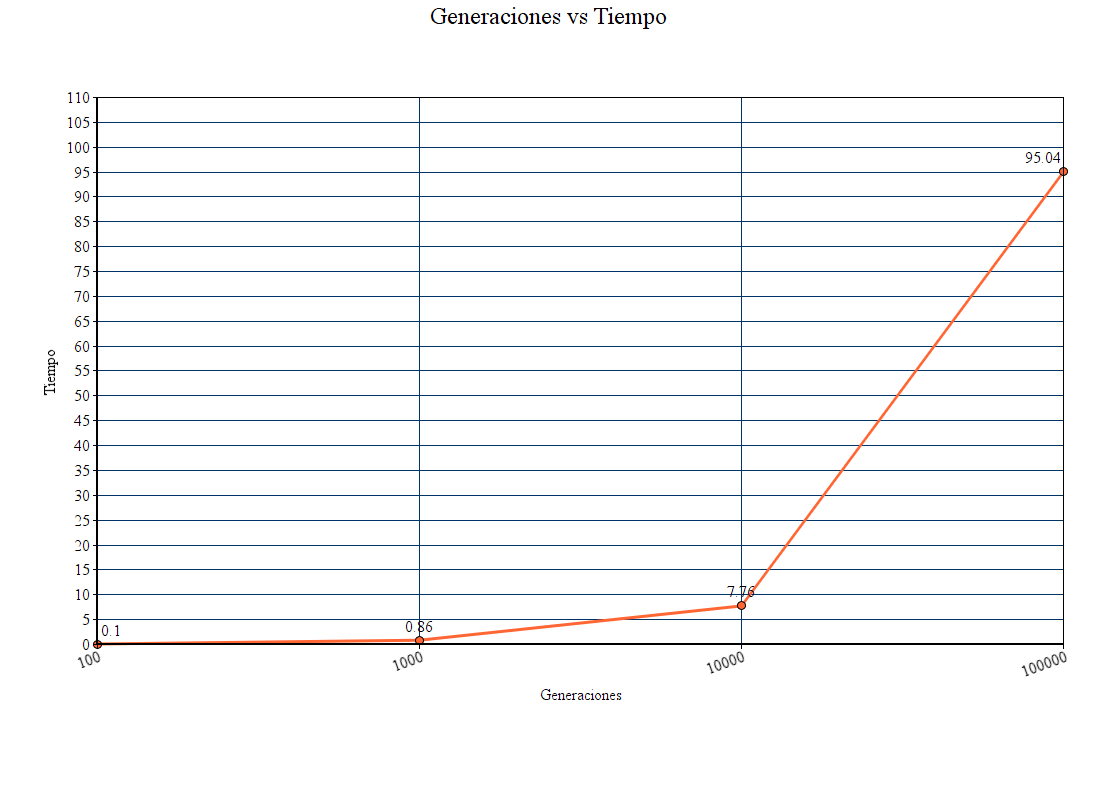
\includegraphics[scale=0.3]{GenVsTiempo.png}
\caption{Grafico de tiempo de ejecución versus cantidad de generaciones. Fuente: Elaboración Propia.}
\label{fig:genvstime}
\end{figure}

Con todos los otros parámetros seleccionados, se pasó a probar uno de los parámetros más influyentes, la cantidad de iteraciones que realiza el algoritmo, eso quiere decir la cantidad de Generaciones (ver Cuadro \ref{tab:generations}).

Se observó que mientras mayor es la cantidad de Generaciones, se encuentra una mejor solución, pero el tiempo de ejecución del programa aumenta exponencialmente (ver Figura \ref{fig:genvstime}). Utilizano el algoritmo implementado se obtuvieron mejores resultados que \cite{bish2011planning}, con la función objetivo min-max, pero como no se sabe que método utiliza el software utilizado por \cite{bish2011planning}, no podemos realizar una buena comparación.



\section{Conclusiones}
%De acuerdo a la introducci\'on que se hizo, entregar afirmaciones RELEVANTES basadas en los experimentos
%y sus resultados.

El Bus Evacuation Problem, es un problema que por sus características resulta muy útil para nuestro país, ya que nuestro país en los últimos años ha tenido una gran cantidad de catástrofes. 

Como este problema es relativamente reciente no existe gran cantidad de literatura acerca de él, sus variantes aunque son pocas buscan acercarse más a la realidad, agregando incertidumbre que es algo inherente a un momento de emergencia, pero todavía falta mucho por trabajar, ya que en los modelos se toman muchos supuestos que en realidad no siempre se cumplen, como por ejemplo la simetría de los trayectos, puede ser que como todos los autos estan evacuando es más fácil volver desde un refugio a un punto de reunión que viceversa por culpa de la congestión. Además como estamos tratando con gente con movilidad reducida, puede ser que necesiten buses especiales, y llegar a lugares especializados, lo que podría aumentar la complejidad del problema.

En la literatura del BEP, se han utilizado variadas técnicas para resolverlo, algunas más completas como la programación lineal, y otras utilizando heurísticas, como la implementación de una búsqueda tabú, pero no se han realizado esfuerzos para resolverlo mediante la técnica propuesta en este documento, como son los algoritmos evolutivos, por lo que esta propuesta es un aporte sustancial a la literatura del problema.

En el caso del algoritmo implementado, se puede concluir que la técnica utilizada es muy eficaz y eficiente para encontrar buenas soluciones, encontrando mejores soluciones que las descritas en la literatura, en muy poco tiempo, en algunos casos puntuales, la mejor solución que encuentra es al incializar la población. 

Pero todavia existe mucho por hacer para mejorar este algoritmo, como buscar algún operador de recombinación más eficiente que genere mayor cantidad de soluciones factibles.

\section{Bibliograf\'ia}
\bibliographystyle{plain}
\bibliography{Referencias}
\end{document} 
